\documentclass[9pt]{beamer}
\usetheme{TUDOplain}
% workaround: provide commands not defiend by all bibtex styles
\providecommand{\btxandlong}{und}
\providecommand{\newblock}{}

\usepackage{pgfpages}
\setbeameroption{hide notes}

% link for how to present on mac with skim:
% https://gist.github.com/andrejbauer/ac361549ac2186be0cdb

% sourcing images
\providecommand{\source}{\\ \footnotesize \tugreen{Source:} \footnotemark}
\providecommand{\sourcefix}[1]{\\ \footnotesize \tugreen{Source:} [#1]}

\renewcommand{\caption}[1]{\\ \footnotesize{\captiongrey{#1}}}

\usepackage[english]{babel}
\usepackage[style=authortitle]{biblatex}
\addbibresource{../bibliography.bib}

% reformat footnotes very plain
\makeatletter
\renewcommand\@makefnmark{%
[\@thefnmark]}
\renewcommand\@makefntext[1]{%
  \noindent\tiny [\@thefnmark] #1}
\makeatother
% command for citing
\providecommand{\fcite}[1]{\footcite{#1}}
%

% basic utils
\usepackage[utf8]{inputenc}
\usepackage{enumerate}
\usepackage{graphicx}
\graphicspath{{../images/}}

\AtBeginSection[]{
  \begin{frame}
  \note[item]{placeholder}
  \vfill
  \centering
  \begin{beamercolorbox}[sep=8pt,center,shadow=true,rounded=true]{title}
    \usebeamerfont{title}\insertsectionhead\par%
  \end{beamercolorbox}
  \vfill
  \end{frame}
}

\usepackage{ifthen}
\usepackage{calc}
\usepackage{amsmath,amsfonts,amssymb}
\setbeamertemplate{navigation symbols}{}
%\setbeamertemplate{footline}{}
%\setbeamertemplate{footline}[frame number]{}
\setbeamertemplate{footline}{\small \vspace{-1ex} \vbox{ \insertframenumber /\inserttotalframenumber}}
%\setbeamertemplate{footline}{\fontsize{7pt}{7pt}\selectfont \vspace{-1ex} \vbox{ \insertframenumber /\inserttotalframenumber}}

\author{Matthias Jakobs}
\title{End-to-end Human Activity Recognition framework on Complex Video Datasets \\ Midterm presentation}
\date{\today}
\institute[TU Dortmund]{Pattern Recognition In Embedded Systems,\\ Department of Computer Science \\ LS XII, Technische Universität Dortmund}
%
% frame command
\newenvironment{myframe}[1][]{%
\begin{frame}%
\frametitle{#1}
% start footnote numbers with 1
\setcounter{footnote}{0}


}{%
\end{frame}%
}

\begin{document}
\begin{frame}

\titlepage

\end{frame}

\section{Motivation}
\begin{myframe}[Motivation]
    \begin{itemize}
        \item Present problem
        \item Approach by Luvizon
    \end{itemize}
\end{myframe}

\tableofcontents

\section{Method}

\begin{myframe}[Method - Joint methods]
    \note[item]{Handlungserkennung und Posenbestimmung gemeinsam trainieren. Idee: Profitieren voneinander}
    \note[item]{ Pretraining von Pose (Verschiedene Datensätze für Pose und Action)}
    \note[item]{Optimierung (fine-tuning) passiert end-to-end}
    \note[item]{}
    \note[item]{Oft ist die Ausgabe von neuronalen Netzen zur Posenbestimmung eine Heatmap. Heatmap stellt Softmaxverteilung da}
    \note[item]{\textbf{Argmax als postprocessing schritt nötig} damit exakte Koordinaten. Wenn man end-to-end trainieren will ist ein nicht-differentierbares Argmax aber problematisch.}
    \note[item]{Normalisierte Version des Erwartungswerts des Softmax in x und y Dimension}
	\begin{columns}[T]
	\begin{column}{.45\textwidth}
		\begin{itemize}
			\item \textbf{Multitask Deep HAR}\footnotemark
			\begin{itemize}
                \item Jointly train pose and action recognition
                \item Pre-train pose estimation part, then fine-tune end-to-end
				\item \textit{Soft-argmax}\footnotemark~makes end-to-end learning possible
			\end{itemize}
		\end{itemize}
        \begin{figure}
            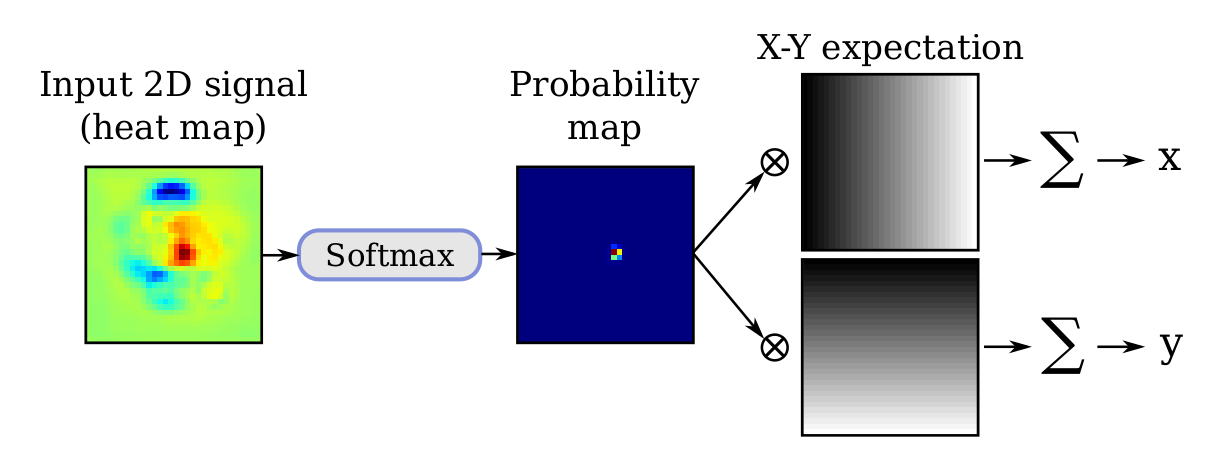
\includegraphics[width=0.99\textwidth]{softargmax.png}
            \sourcefix{1}
        \end{figure}
	\end{column}
    \footnotetext[1]{\cite{luvizon_2d/3d_2018}}
    \footnotetext[2]{\cite{luvizon_human_2017}}
	\begin{column}{.45\textwidth}
		\begin{figure}
			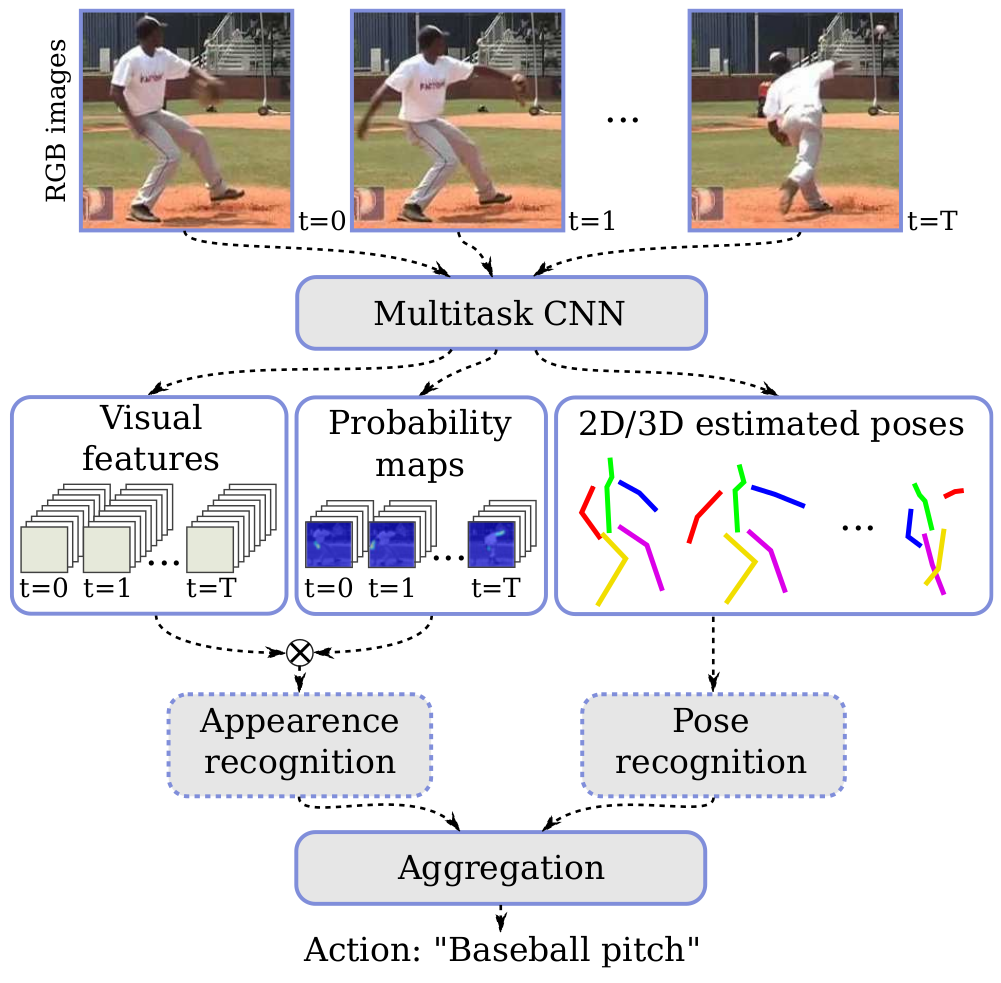
\includegraphics[width=.99\textwidth]{endtoend-concept.png}
            \sourcefix{1}
            %\caption{Complete network pipeline.}
		\end{figure}
	\end{column}
	\end{columns}
\end{myframe}

\begin{myframe}[Multitask Deep HAR - Architecture]
    \note[item]{Basiert auf Inception v4 um Features zu extrahieren}
    \note[item]{Prediction Blocks: Ähnlich zu Hourglasses von vorhin. Nach jedem Block ein Zwischenergebnis welches verfeinert wird.}
    \note[item]{Nach \textbf{jedem} prediction block: Heatmap (Softargmax) und Wahrscheinlichkeitsvektor}
    \note[item]{Loss: Elstic Net loss}

    \begin{columns}[T]
        \begin{column}{.45\textwidth}
            \begin{itemize}
                \item \textit{Multitask CNN}
                \begin{itemize}
                    \item Blocks similar to hourglasses
                    \item Refine prediction with each additional block
                    \item In addition to providing visual features and heatmaps:
                    \begin{itemize}
                        \item Coordinates from Soft-argmax
                        \item Join visibility vector using sigmoid
                    \end{itemize}
                    \item Loss function $$L_p = \frac{1}{N_J}\sum_{n=1}^{N_J}(~ \lvert\lvert \hat{p}_n - p_n \rvert\rvert_1 ~+~ \lvert\lvert \hat{p}_n - p_n \rvert\rvert^2_2 ~ )$$
                \end{itemize}
            \end{itemize}
        \end{column}
        \begin{column}{.45\textwidth}
            \begin{figure}
                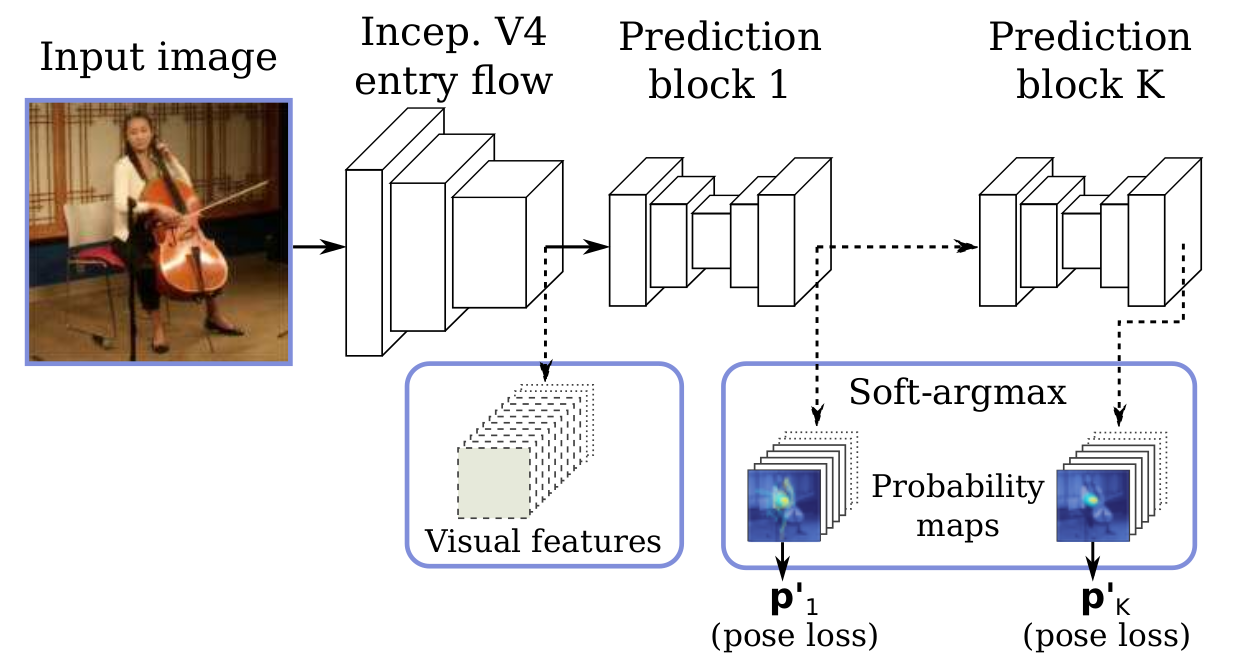
\includegraphics[width=.99\textwidth]{multitask-part.png}
                \sourcefix{1}
            \end{figure}
        \end{column}
	\end{columns}
    \footnotetext[1]{\cite{luvizon_2d/3d_2018}}
\end{myframe}

\begin{myframe}[Multitask Deep HAR - Architecture]
    \note[item]{Pipeline zu sehen.}
    \note[item]{Auch hier: keine genauen Angaben zum Aufbau. Verweis auf Code}
    \note[item]{Action Heatmap für jede Handlung. Mittles Pooling und Softmax dann Wahrscheinlichkeit}
    \note[item]{Max+Min pooling: $f(x) = \text{MaxPooling}(x) - \text{MaxPooling}(-x)$}

	\begin{columns}[T]
        \begin{column}{.45\textwidth}
            \begin{itemize}
                \item \textit{Pose recognition}
                \begin{itemize}
                    \item Arrange joint values over time in 2D matrix
                    \item Action heatmaps
                    \begin{itemize}
                        \item Through softmax: action probabilities
                    \end{itemize}

                \end{itemize}
            \end{itemize}
        \end{column}
        \begin{column}{.45\textwidth}
            \begin{figure}
                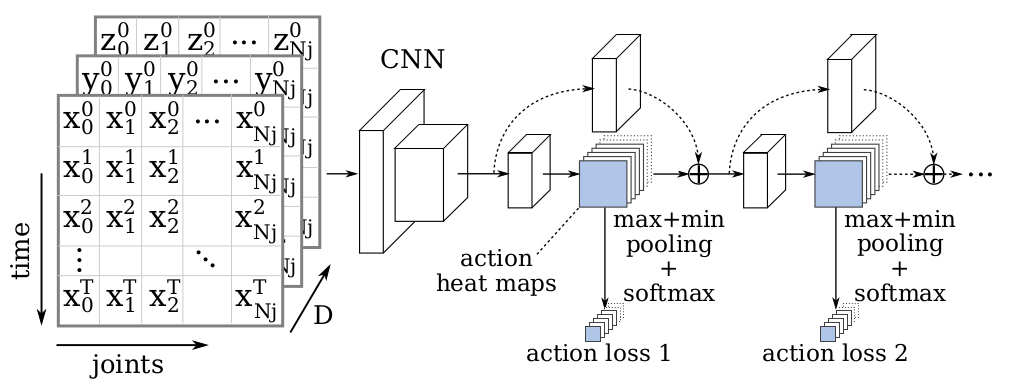
\includegraphics[width=.99\textwidth]{jointsovertime.png}
                \sourcefix{1}
            \end{figure}
        \end{column}
	\end{columns}
    \footnotetext[1]{\cite{luvizon_2d/3d_2018}}
\end{myframe}

\begin{myframe}[Multitask Deep HAR - Architecture]
    \note[item]{Im Prinzip gleicher Aufbau wie vorher, nur mit Visual Features statt Posen}
    \note[item]{\textbf{Am Ende:}}
    \note[item]{Durch FC-Layer aggregation und mit softmax dann finales Ergebnis}
	\begin{columns}[T]
        \begin{column}{.45\textwidth}
            \begin{itemize}
                \item \textit{Appearance recognition}
                \begin{itemize}
                    \item Combination of visual features and joint positions
                    \item Then: Identical architecture to pose recognition part
                \end{itemize}
                \item \textit{Aggregation}
                \begin{itemize}
                    \item Combine pose recognition and appearance recognition for final result
                    \item \textit{Categorical cross-entropy}
                \end{itemize}
            \end{itemize}
        \end{column}
        \begin{column}{.45\textwidth}
            \begin{figure}
                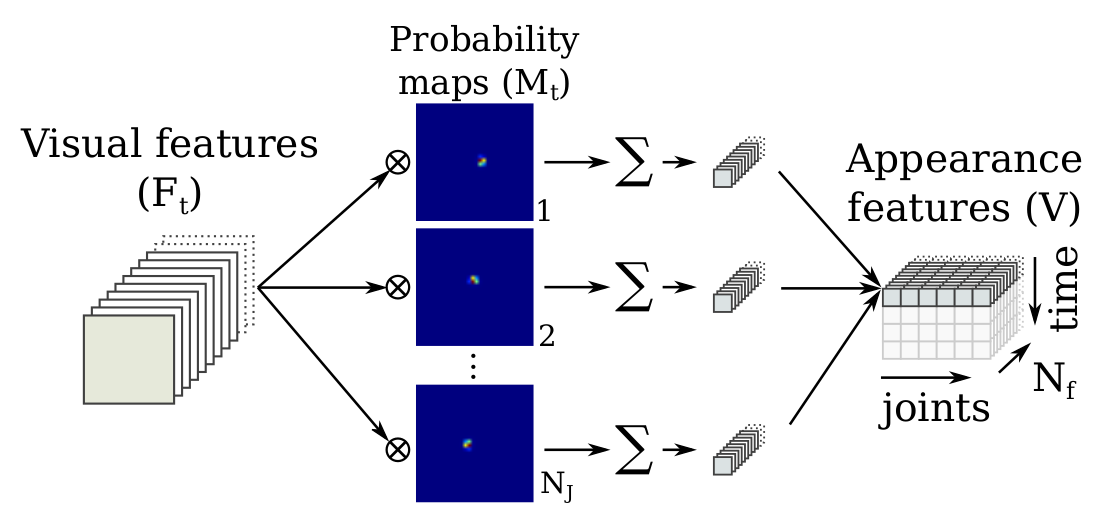
\includegraphics[width=.99\textwidth]{appearance-features.png}
                \sourcefix{1}
            \end{figure}
        \end{column}
	\end{columns}
    \footnotetext[1]{\cite{luvizon_2d/3d_2018}}
\end{myframe}

\begin{myframe}[Method]
    \note[item]{placeholder}
    \begin{itemize}
        \item Reimplementation in PyTorch \fcite{paszke_automatic_2017}
        \begin{itemize}
            \item Evaluate against JHMDB \fcite{jhuang_towards_2013}
        \end{itemize}
        \item Experimentation
        \begin{itemize}
            %\item Better incorporation of temporal dimension \fcite{pavllo_3d_2019}
            \item Compare with state-of-the-art methods not using pose \fcite{zhou_mict:_2018}
            \item Different representation of temporal information (next slide)
            \item Combined loss function of pose and action for \emph{real} end-to-end training
        \end{itemize}
    \end{itemize}
\end{myframe}

\begin{myframe}[Method]
    \note[item]{Dadurch: Eine Repräsentation für Video features und IMU Datenströme. \textit{Kombination?}}
    \begin{figure}
        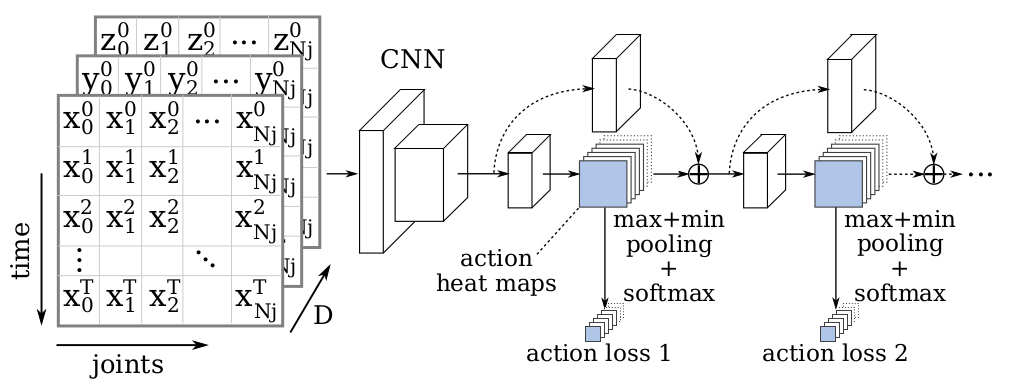
\includegraphics[width=.65\textwidth]{jointsovertime.png}
        \caption{Approach used by \footnotemark. Convolution over all sensors at once. \sourcefix{1}}
    \end{figure}
    \begin{figure}
        \includegraphics[width=.65\textwidth]{sensor-time.png}
        \caption{Impression of pixel coordinates of joints over time \source}
    \end{figure}
    \footnotetext[1]{\cite{luvizon_2d/3d_2018}}
    \footnotetext[2]{\url{https://avtech.com/articles/wp-content/uploads/2015/06/Intro.-Pic.png}}
\end{myframe}

\section{Datasets}
\begin{myframe}[2D Pose Datasets]
  \note[item]{placeholder}
  \begin{columns}[T]
      \begin{column}{.48\textwidth}
          \begin{itemize}
              \item \textbf{MPII Human Pose\footnotemark}
              \begin{itemize}
                  \item 40,000 annotated images
                  \item Single and multi person
                  \item Over 401 different activities
              \end{itemize}
          \end{itemize}
      \end{column}
      \footnotetext[1]{\cite{andriluka_2d_2014}}
      \begin{column}{.48\textwidth}
          \begin{figure}
              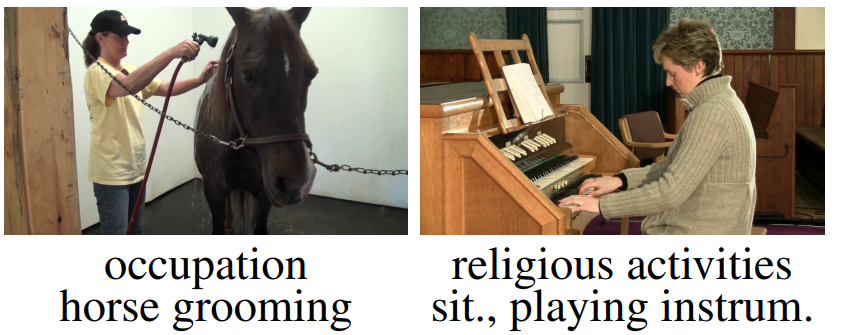
\includegraphics[width=0.99\textwidth]{mpii.png}
              \sourcefix{1}
          \end{figure}
      \end{column}
  \end{columns}
\end{myframe}


\begin{myframe}[Action Recognition Datasets]
  \note[item]{placeholder}
  \begin{columns}[T]
      \begin{column}{.48\textwidth}
          \vspace{20px}
          \begin{itemize}
              \item \textbf{Penn Action\footnotemark}
              \begin{itemize}
                  \item 2,400 video clips of 15 actions
                  \item Very limited number of actions (mainly sport)
              \end{itemize}
          \end{itemize}
      \end{column}
      \footnotetext[1]{\cite{zhang_actemes_2013}}
      \begin{column}{.48\textwidth}
          \begin{figure}
              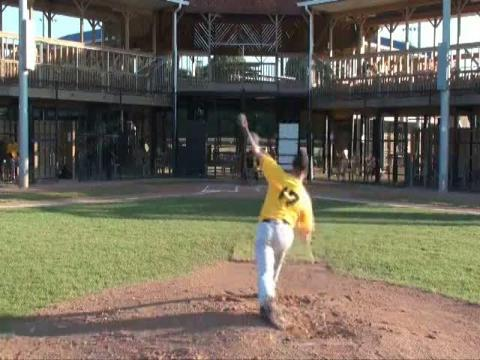
\includegraphics[height=45px]{pa-01.jpg}
              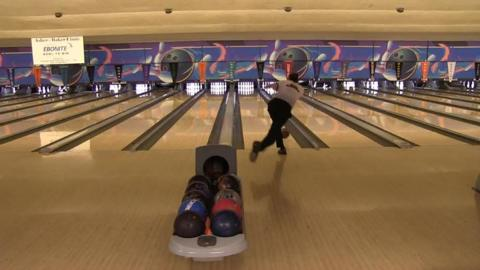
\includegraphics[height=45px]{pa-02.jpg}
              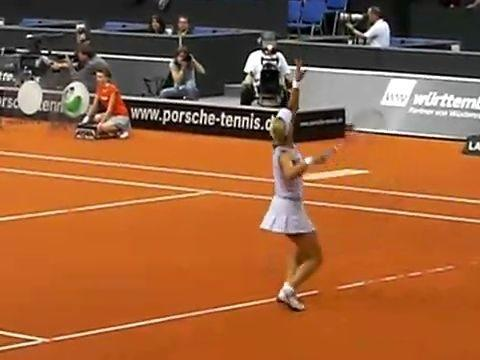
\includegraphics[height=45px]{pa-03.jpg}
              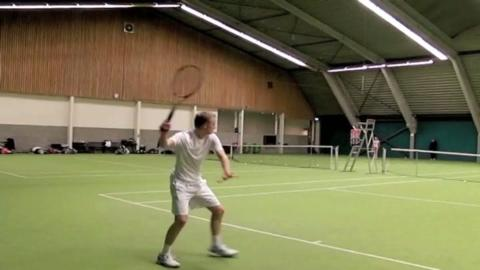
\includegraphics[height=45px]{pa-04.jpg}
              \source
          \end{figure}
      \end{column}
  \end{columns}
  \footnotetext[2]{\url{https://upenn.app.box.com/v/PennAction}}
\end{myframe}

\begin{myframe}[Action Recognition Datasets]
  \note[item]{placeholder}
  \begin{columns}[T]
      \begin{column}{.48\textwidth}
          \begin{itemize}
              \item \textbf{JHMDB\footnotemark}
              \begin{itemize}
                  \item Fully-annotated subset of HMDB
                  \begin{itemize}
                      \item 2D pose, person segmentation maps etc.
                  \end{itemize}
                  \item 928 clips of 21 actions
                  \item Can be used for end-to-end training
              \end{itemize}
          \end{itemize}
      \end{column}
      \footnotetext[1]{\cite{jhuang_towards_2013}}
      \begin{column}{.48\textwidth}
          \begin{figure}
              \includegraphics[height=.55\textheight]{jhmdb.png}
              \centering
              \source
          \end{figure}
      \end{column}
  \end{columns}
  \footnotetext[2]{\url{http://jhmdb.is.tue.mpg.de/puppet_tool}}
\end{myframe}

\section{Experiments}
\begin{myframe}[Recreate experiments]
    \begin{itemize}
        \item MPII in all different kinds
        \item Show example images and graphs
    \end{itemize}
\end{myframe}

\begin{myframe}[Recreate experiments]
    \begin{itemize}
        \item Penn Action HAR
        \item Show example images and graphs
    \end{itemize}
\end{myframe}

\section{Conclusion}
%\note[item]{placeholder}
\begin{myframe}[Conclusion]
    \begin{itemize}
        \item TODO
    \end{itemize}
\end{myframe}

\begin{myframe}[Thank you]
    \note[item]{placeholder}
    \centering \Large
    \emph{Thank you for your time!}
\end{myframe}

\end{document}

